\documentclass{article}
\topmargin 0pt
\advance \topmargin by -\headheight
\advance \topmargin by -\headsep
\textheight 8.9in
\usepackage{color}
\usepackage{amsmath}
\usepackage{amsfonts}
\usepackage[noae]{Sweave}
\usepackage{enumerate}
\oddsidemargin 0pt
\evensidemargin \oddsidemargin

\begin{document}
\title{ CSCI-B 565 DATA MINING \\
Homework 4 \\
Morning Class\\
Computer Science Core\\Fall 2013\\Indiana University}
\author{ Debpriya Seal\\ debseal@indiana.edu}
\maketitle
All the work herein is solely mine. \\

\section*{Problem One}
		Fraudulent Sales Data\\
	\emph{Answer:} 
	\begin{enumerate}
		\item \textbf{Description for Layman:}
		This is a problem in which we were given with sales transactions (of products) which a salesman make on a daily basis. However, it is beilieved by the company owners that few saleman does put some transactions of product which never happened. The data mining task is to come up with an algorithm to analyze this data and tell the owner of the company that which transaction could be fraud. Which they will go ahead to scrutinize. This way company do not need to check each and every transaction of each and every employee/salseman.

		\item \textbf{Description for computer Scientist:}
		The problem in hand is that of classification.We are given with a dataset comprised of the daily sales transactions by various sale representative of a company. Looking at the transactions company see some fraud transactions taking place. The company provided us with dataset in which they did identified so fraud transacitons and similarly for normal/OK transaction. However, as expected they could not go through all the transaction and they are labeled as "Unkn" in the dataset. The task is to help them narrow down the transactions they need to scrutinze for fraud dectection.
		\item Analysis of original data $\Delta$\\
		\emph{Answer:} After my analysis of data, below are my findings:
		\begin{enumerate}
			\item At the first glance, when you see Quantity and Value, immediatly Unit price of the products comes to 	mind.As it can be an interesting feature for classification.
			\item For unit price computation, we have missing values for 2 columns Quant and Values.Cases where one of them is missing and when both are missing.
			\item For trainig purposes, we have only approx. $4\%$ of the total data. Which is not huge.Plus we can see imbalance in the training data as number of transactions with "OK" is much higer than "Fraud".
			\item If we see the number of transactions done by any salesman. It has huge difference as expected. Since depending on the city salesman stays his sales would be effect.Similarly, we see teh frequency of the sale, we see that there is again huge difference, much to our expectation. As few products may be more popular than others.
			\item One interesting statistic is, the top 100(in terms of number of sales) salesman account for the $40\%$ of he sale of the company. Similarly, top 100 products(in terms of price) accounts for the $75\%$ of the sale. However, this statistics is not that interesting as they might have higher margin over the low price products.
			\item There are few products for which for all the transcations either quanity or values are missing. Yet they have the Insp being tagged as OK/Fraud. This indicate typing errors or the person inspecting has additional knowledge.
		\end{enumerate}

		\item Steps to clean and transform data to  $\Delta$*\\
		\emph{Answer:}  Below are the steps which I took to clean the data:
		\begin{enumerate}
			\item Firstly, I computed the Unit Price for transaction in which both Quantity and Values are present.And then computed the typical unit Price $(UnitPrice)$ of a product by taking the \textbf{Median} of those unit Prices.
			\item For the case when Quantity is missing. I looked into the typical $UnitPrice$ for that product. Divided values of that product with  $UnitPrice$ to get the missing Quanity. Took $Math.ceil$ to make sure I get round figure.
			\item For the case when Values is missing. I looked into the typical $UnitPrice$ for that product. Multiplied quantity of that product with  $UnitPrice$ to get the missing Values. Took $Math.ceil$ to make sure I get round figure.
			\item Cases when both are missing. I just dropped those records.
			\item Cases when for a particular product all the transcations had either Quantity or Values missing.I dropped them as well.
		\end{enumerate}
\textbf{Snapshot from my program output:}\\
++++++++++++++++++++++++++++\\
Cleaning Data..........\\
++++++++++++++++++++++++++++\\
Number of records post dropping records with missing values: 400204\\
Number of records with both qty and val missing: 942\\
Computing Unit price....\\
Number of records for which Qty value replaced: 12900\\
Number of records for which val value replaced: 294\\
		\item Data Mining algorithms employed (and implemented, of course) to solve $\Delta$\\
		\emph{Answer:} Below are the 3 algorithms implemented to solve $\Delta$
		\begin{enumerate}
			\item Navie Bayes: I implemented this algorithm to classify the transaction as "Fraud", "OK". Naive Bayes is works well with discrete attributes. However, in the present dataset we have one attribute is continous. To resolve this problem, I have assumed that the distribution of UnitPrice is normally distributed and computed the p(x) by below formula: \\
$p(x) = \frac{1}{\sigma \sqrt{2 \pi }}  \mathrm{e}^{-\frac{(x- \mu)^2}{2\sigma^2}}$

			\item k Means: Fo K means clearly, the k would be 2 as we are trying to cluster transactions into two cluster one for Fraud and other for OK.  I am using the eculidean distance as my metric. And I am presuming that the smaller cluster is the one which one is fraud and the other one is OK. As the number of transaction being fraud has less probabililty than OK.

			\item IterativeDichotomiser3: ID3 is again a classification algorithm that I have used. And like Naive Bayes  continous attribute even here comes up as an hurdle. Since, its been seen emperically that ID3 works poorly with continuos attributes. So we need to discretize it. So for this I sorted the UnitPrice checked for the change in class and picked the one with highest information gain.
		\end{enumerate}
		
		\item Quality of results. \\
		\emph{Answer:} Below are the results from my 3 different classification algorithms:
		\begin{enumerate}
			\item Navie Bayes:
			\begin{Sinput}
Number of transaction classified as Fraud:	2202
Number of transaction classified as OK:	382276
			\end{Sinput}
			\item k Means:
			\begin{Sinput}
Number of transaction classified as Fraud:	2202
Number of transaction classified as OK:	382276
			\end{Sinput}
			\item IterativeDichotomiser3:\\
Attr Picked in Order:	[ID, UPrice, Prod]\\
+++++++++++++++++++++++++++++++++++++\\
Your Decision Tree looks like below: Parent: [child1,child2,... ]
+++++++++++++++++++++++++++++++++++++\\
ID:[UPrice, Prod, ok, ok, ok, ok, ok, ok, ok, ok, ok, ok, ok, ok, ok, ok, ok, ok, ok, ok, ok, ok, ok, ok, ok, ok, ok, ok, ok, ok, ok, ok, ok, ok, ok, ok, ok, ok, ok, ok, ok, ok, ok, ok, ok, ok, ok, ok, ok, ok, ok, ok, ok, ok, ok, ok, ok, ok, ok, ok, ok, ok, ok, ok, ok, ok, ok, ok, ok, ok, ok, ok, ok, ok, ok, ok, ok, ok, ok, ok, ok, ok, ok, ok, ok, ok, ok, ok, ok, ok, ok, ok, ok, ok, ok, ok, ok, ok, ok, ok, ok, ok, ok, ok, ok, ok, ok, ok, ok, ok, ok, ok, ok, ok, ok, ok, ok, ok, ok, ok, ok, ok, ok, ok, ok, ok, ok, ok, ok, ok, ok, ok, ok, ok, ok, ok, ok, ok, ok, ok, ok, ok, ok, ok, ok, ok, ok, ok, ok, ok, ok, ok, ok, ok, ok, ok, ok, ok, ok, ok, ok, ok, ok, ok, ok, ok, ok, ok, ok, ok, ok, ok, ok, ok, ok, ok, ok, ok, ok, ok, ok, ok, ok, ok, ok, ok, ok, ok, ok, ok, ok, ok, ok, ok, ok, ok, ok, ok, ok, ok, ok, ok, ok, ok, ok, ok, ok, ok, ok, ok, ok, ok, ok, ok, ok, ok, ok, ok, fraud, fraud, fraud, fraud, fraud, fraud, fraud, fraud, fraud, fraud, fraud, ok, ok, ok, ok, ok,......, fraud, fraud, fraud, fraud, fraud, ok, ok]\\
\\ UPrice:[ok, ok, ok, ok, ok, ok, ok, fraud, fraud]\\
\\ Prod:[ok, ok, ok, fraud, ok, ok, ok, ok, ok]\\
\\ ok:[]\\
\\ fraud:[]\\
		\end{enumerate}

		\item Analysis of results that includes suggestion of what, if anything, can be done w.r.t. $\Delta$\\
		\emph{Answer:} One suggestion I would like to give is to have volume of data for different class to be of  nearly size. As otherwise it present various problems for the classfication task. As the data mining algorithm may ignore this class with smaller size given not enough information about it. And it is very bad for us, as we are more interested in them only.

		\item Appendix that includes code, citations (if any), links, etc.\\
		\emph{Answer:} Please refer to Reference Section.
	\end{enumerate}	


\section*{Problem Two} You've received a strange data set enigma.txt. Analyze the data.\\
	\emph{Answer:} \emph{\textbf{My Analysis Of Data}}: \\
	As per may anaylsis I assumed the $1^{st}$ column to be a YYYY.MM format. And $2^{nd}$ column to be a value for every month. Now that can be anything revenue etc. Below is my analysis in R:
\begin{enumerate}
\item create data frame from file and making 2 columns from 1st column i.e. of Year and month
\begin{Schunk}
\begin{Sinput}
library(ggplot2)
myData <- read.table("engima.txt", sep="",header = FALSE, colClasses=c("character", "numeric"))
year <-substr(myData[,1],0,4)
uniqueYear <-unique(year)
month <- substr(myData[,1],6,nchar(myData[,1]))
monthNum <- as.numeric(unique(month))
factorMonth <- factor(monthNum, levels=monthNum, ordered=TRUE)
myData <- cbind(year, factorMonth, myData[c(-1)])
str(myData)
\end{Sinput}
\begin{Soutput}
'data.frame':	600 obs. of  3 variables:
 $ year       : Factor w/ 50 levels "1945","1946",..: 1 1 1 1 1 1 1 1 1 1 ...
 $ factorMonth: Ord.factor w/ 12 levels "1"<"2"<"3"<"4"<..: 1 2 3 4 5 6 7 8 9 10 ...
 $ V2         : num  18.5 11.8 19.7 31.6 26.6 37.3 37.4 24.6 34 71.3 ...
\end{Soutput}
\begin{Soutput}
head(myData) 

  year factorMonth   V2
1 1945           1 18.5
2 1945           2 11.8
3 1945           3 19.7
4 1945           4 31.6
5 1945           5 26.6
6 1945           6 37.3
\end{Soutput}
\end{Schunk}
\item If we observe the below plot closely, you can see a wave pattern. In the $1^{st}$ row the peak is in middle.However, in the $2^{nd}$ row it shifts. And in the $3^{rd}$ row it shifts completely. If we plot this in a single row you can clearly see that it is following a wave pattern. \\
\begin{Schunk}
\begin{Sinput}
> qplot(data=myData,x=factorMonth,y=V2,color=year, facets =~year, group=year) + 
+ geom_line() + ylab("Values") +xlab("Months")
\end{Sinput}
\end{Schunk}
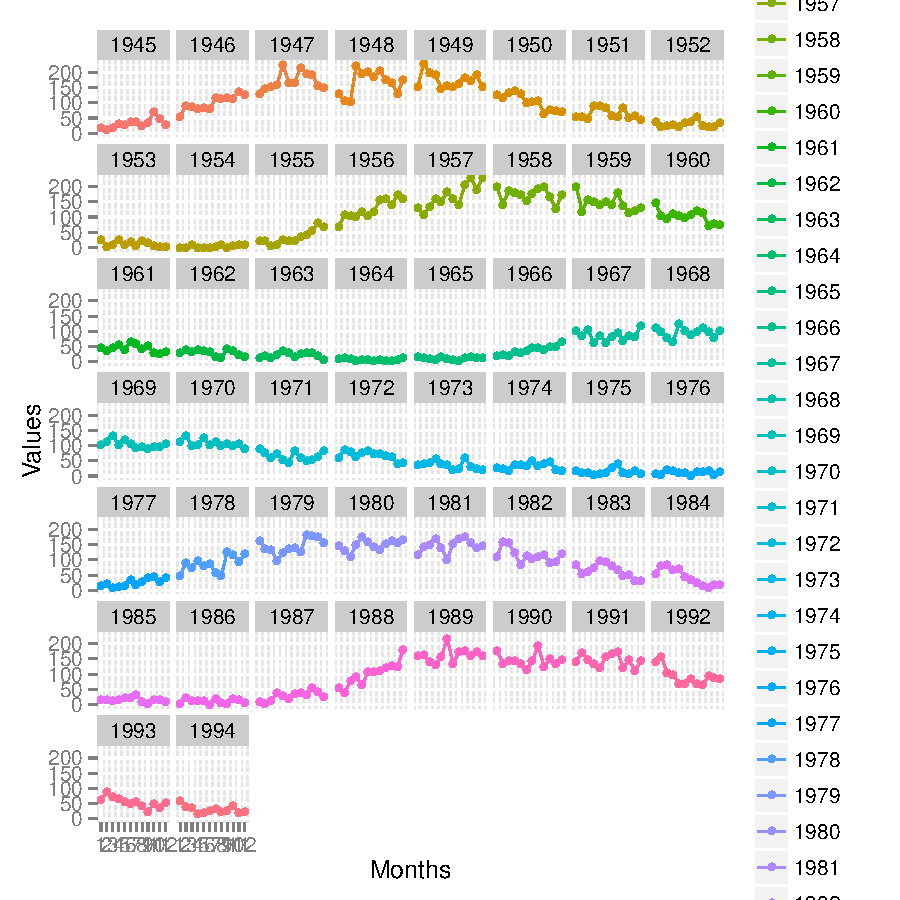
\includegraphics{debseal_HW4-002}
\item This time I plot the data monthwise and again we can see a strong sine pattern even within a year. \\
\begin{Schunk}
\begin{Sinput}
> qplot(data=myData,x=year,y=V2,color=factorMonth, facets =~factorMonth, group=factorMonth) + geom_line() + ylab("Values") +xlab("Years")
\end{Sinput}
\end{Schunk}
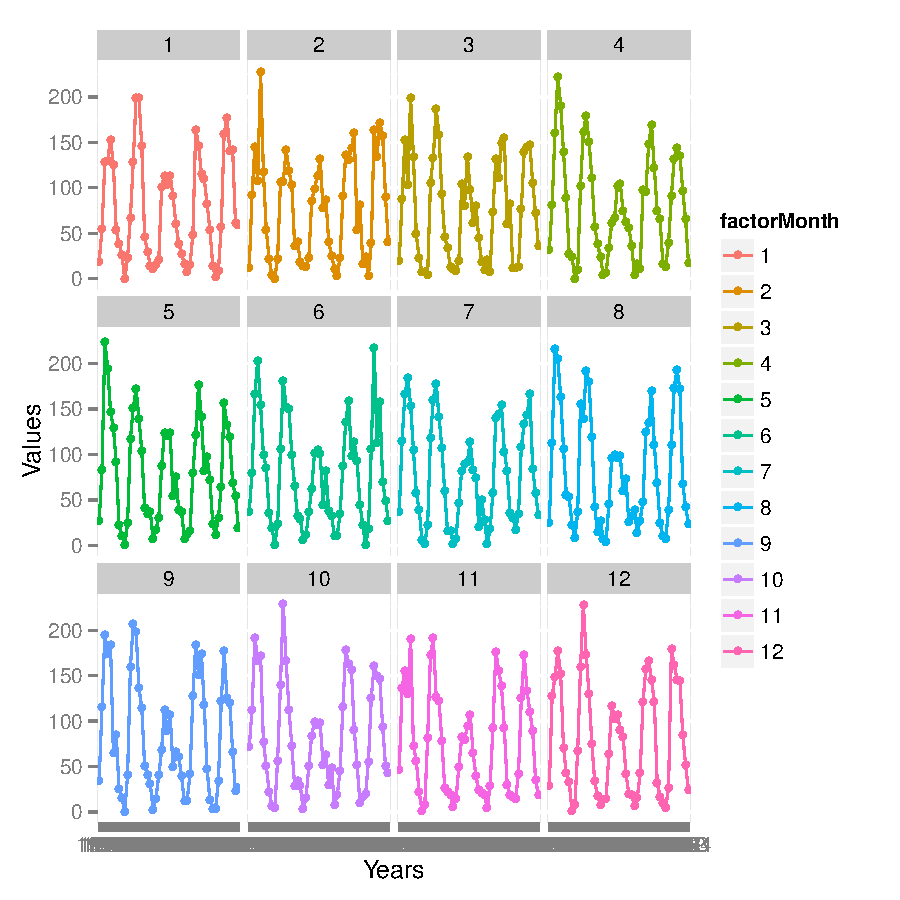
\includegraphics{debseal_HW4-003}
\item This time I went ahead to see the behviour of the median and again the inherent wave pattern comes up.
\begin{Schunk}
\begin{Sinput}
> ggplot(myData, aes(x=year, y=V2)) + 
+   geom_boxplot() + 
+   stat_summary(fun.y=median, geom="line", aes(group=1,color="median", colours="red")) +
+   stat_summary(fun.y=median, geom="line", aes(group=1, color="median"))
\end{Sinput}
\end{Schunk}
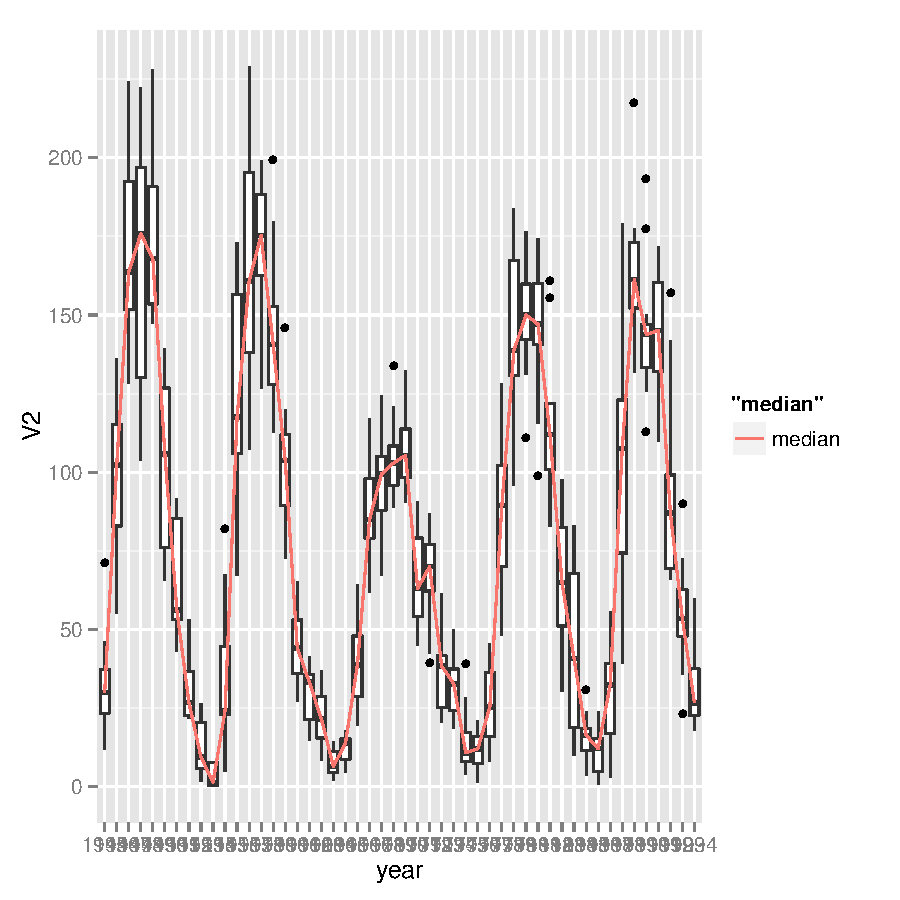
\includegraphics{debseal_HW4-004}
\end{enumerate}
\section*{Problem Three: } I am providing you with voting data from the 35th to the 112th US Congressional Sessions. What can you you say about the differences between Republican and Democratic Members? What about Northern Democrat and Southern Republicans? What about Northern Republican and Southern Democrats? The data is in an *.csv file USCongress. \\
\emph{Answer:} 
\begin{enumerate}
	\item Republican and Democratic Members \\
	\textbf{\emph{For Yes:}}Below 2 screenshot shows clear increase in Number of Yes by both parties:\\
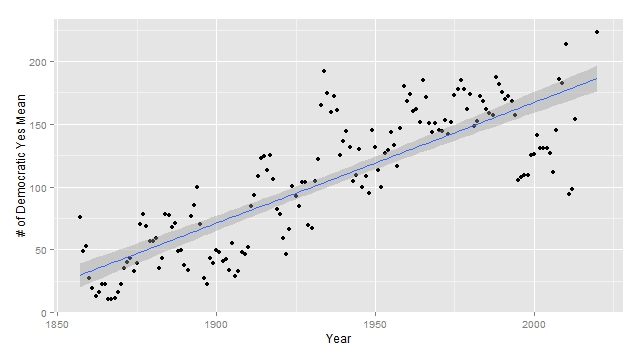
\includegraphics{DemocratYes} \\
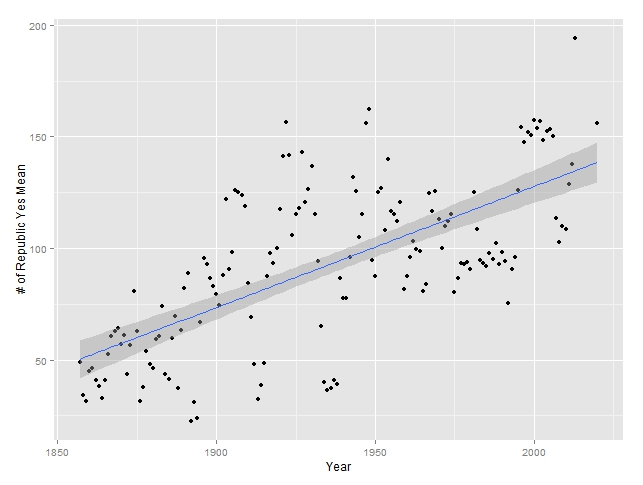
\includegraphics{RepublicYes} \\
	\textbf{\emph{For No:}}However, the number of No' were pretty consistent for both of them.

	\item Southern Republican and Nothern Democratic Members \\
	\textbf{\emph{For No:}}\\
As you can see that lately S Republic has started to increase their number of Nays.\\
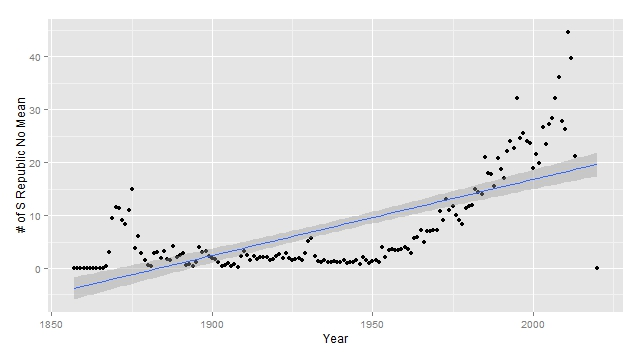
\includegraphics{SRepubNo} \\
 On the other hand, for the Nothern Democratic they increased it pretty uniformly.\\
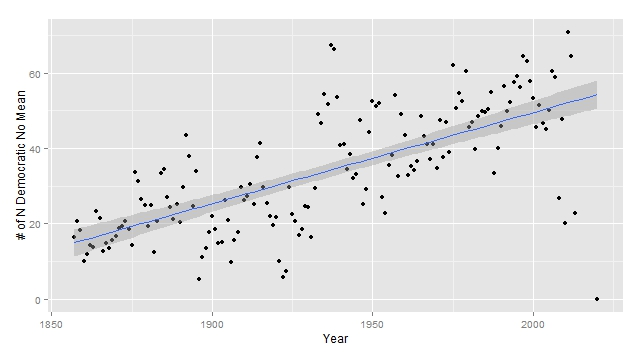
\includegraphics{NorthDemNo} \\

\textbf{\emph{For Yes:}}\\
\textbf{Quite Strangley} Southern Republican and Nothern Democratic mean of YES also follows a smiliar trend as that of NO.\\
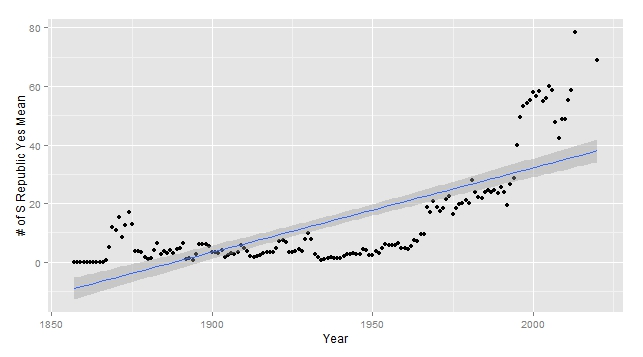
\includegraphics{SRepbYes} \\
	\item Nothern Republican and Southern Democratic Members \\
	\textbf{\emph{For Yes:}}\\
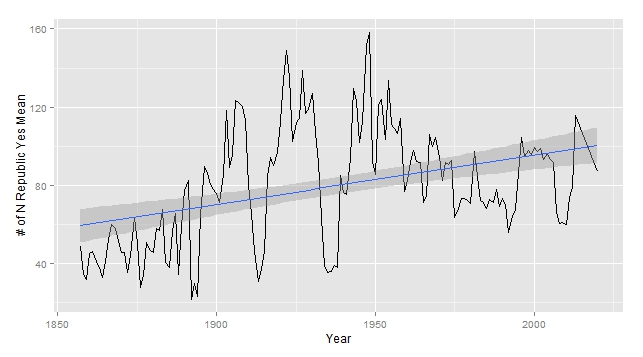
\includegraphics{NRepbYes} \\
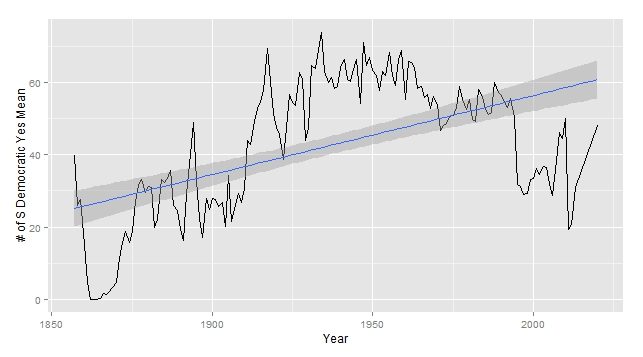
\includegraphics{SDemYes} \\	
	\textbf{\emph{For No:}} \\
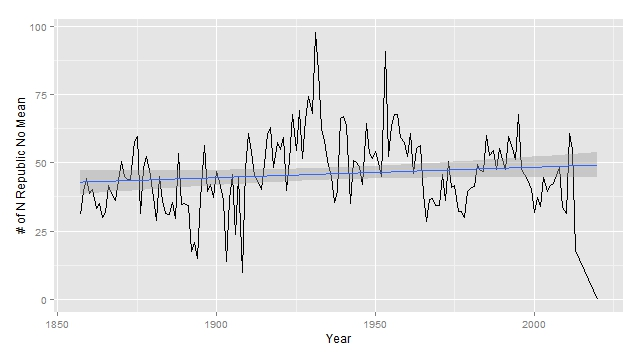
\includegraphics{NRepubNo} \\
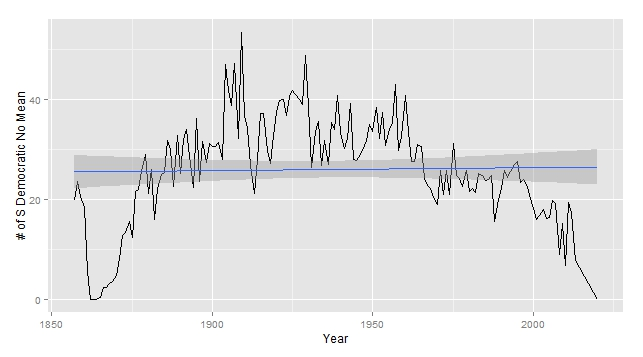
\includegraphics{SDemNo} \\
	\item Missing Votes\\
	Clearly, we see that the count of Missing Votes have dropped over the course of the time.\\
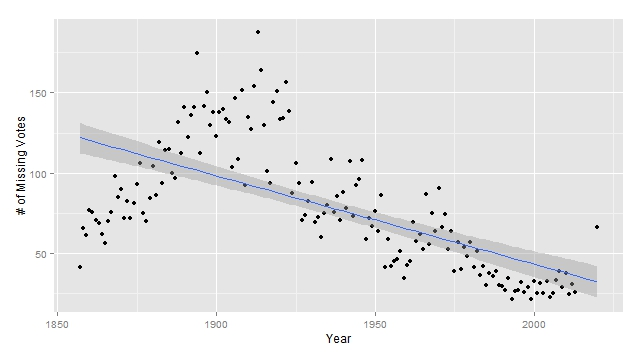
\includegraphics{MissingVotes} \\
\end{enumerate}

\begin{itemize}
	\renewcommand{\labelitemi}{$\bullet$}
	\item Write two reasonably formal statements that use $\Delta$ as either clustering or classification problems.Is the data amenable to both clustering and classification or is one method more appropriate?\\
	\emph{Answer:}
	
	\begin{enumerate}[1.]
		\item Is this a large data set?\\
		\emph{Answer:} Although, large or small is a relative term. However, by any standard any of these are not a huge data set.

		\item Discuss the number of attributes with the data size.\\
		\emph{Answer:}For USCongress we see a huge count. The count of number of attributes is 20. As we know as we go higher in dimension the "curse of high dimension" starts to effect our algorithms. This would be one of the worries for me. 
	\end{enumerate}

	\item Discuss missing values. Perhaps use one of the three methods to replace missing data.Assess the significance of either keeping or removing the tuples with unknown data. Is the amount of missing data significant?\\
	\emph{Answer:} Sales data had quite some misisng values. Although only 888 were such that we had to remove them completly. And it did not seem to be huge. And I have discussed in detail about them as part of first question.
\end{itemize}	
\section*{References}
	\begin{enumerate}
		\item Data Mining with R - Luis Torgo
		\item http://vivin.net/2010/01/30/generic-n-ary-tree-in-java/
	\end{enumerate}
\end{document}
